Known function, simulate input, plot fANOVA and PD, comparison

PD and fANOVA: If inputs are independent, I think for the main effects fANOVA is simply PD shifted but fANOVA answers a different question thatn PD. PD usually asks for the effect of one specific variable on the prediction. In contrast, fANOVA decomposes the entire function. It is more about a global representation and clean, isolated effects because in sum they have to recover the original function and may not overlap.

\subsubsection*{Standard MVN, linear function, interaction}

The plots show the classical fANOVA components for our known example from the previous sections. Classical components visualized, but in this simple example they are simply the subfunctions we can already see from looking at the function.
% include a graphic from image folder right here
% Zwei Plots nebeneinander, jeweils halbe Breite

% Input: MVN, centred, independent
\begin{figure}[htpb]
    \centering
    \begin{minipage}[t]{0.49\textwidth}
        \centering
        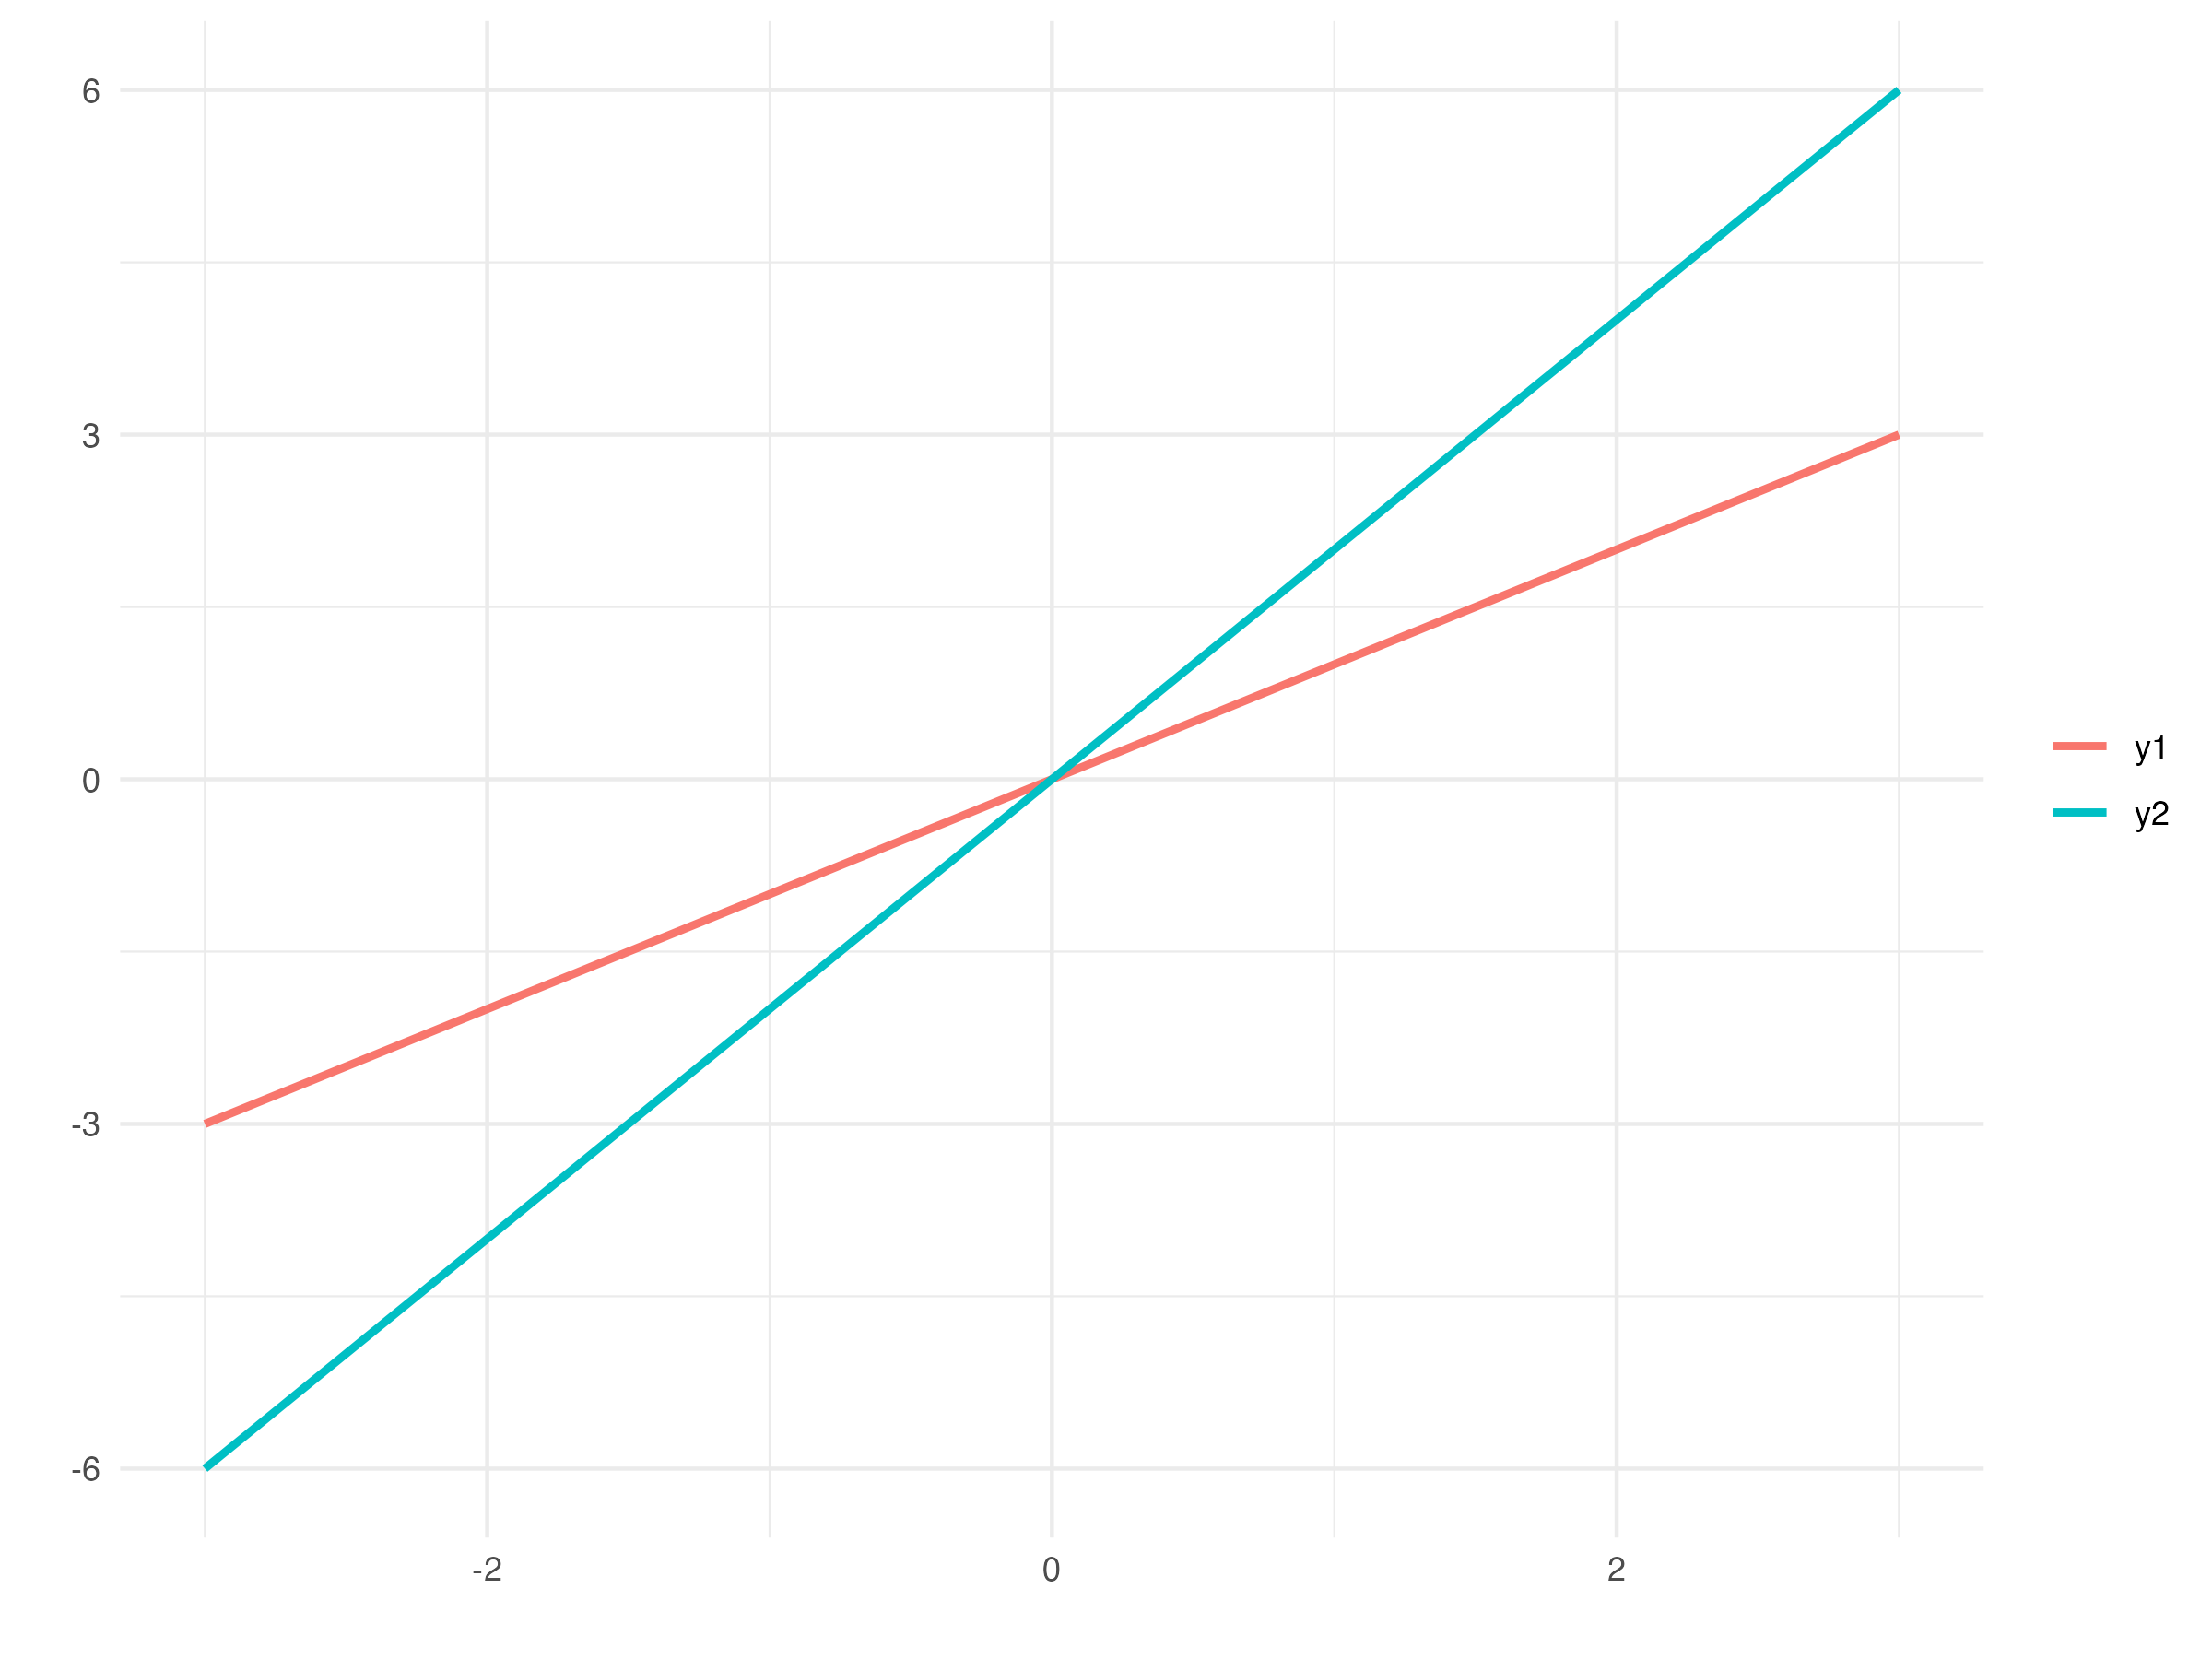
\includegraphics[width=\textwidth]{images/p_main_effect_ex1.png}
        \caption{Main terms as calculated via classical fANOVA for $g(x) = x_1 + 2 x_2 + x_1 x_2$.}
        \label{fig:main_effects_ex1}
    \end{minipage}%
    \hfill
    \begin{minipage}[t]{0.49\textwidth}
        \centering
        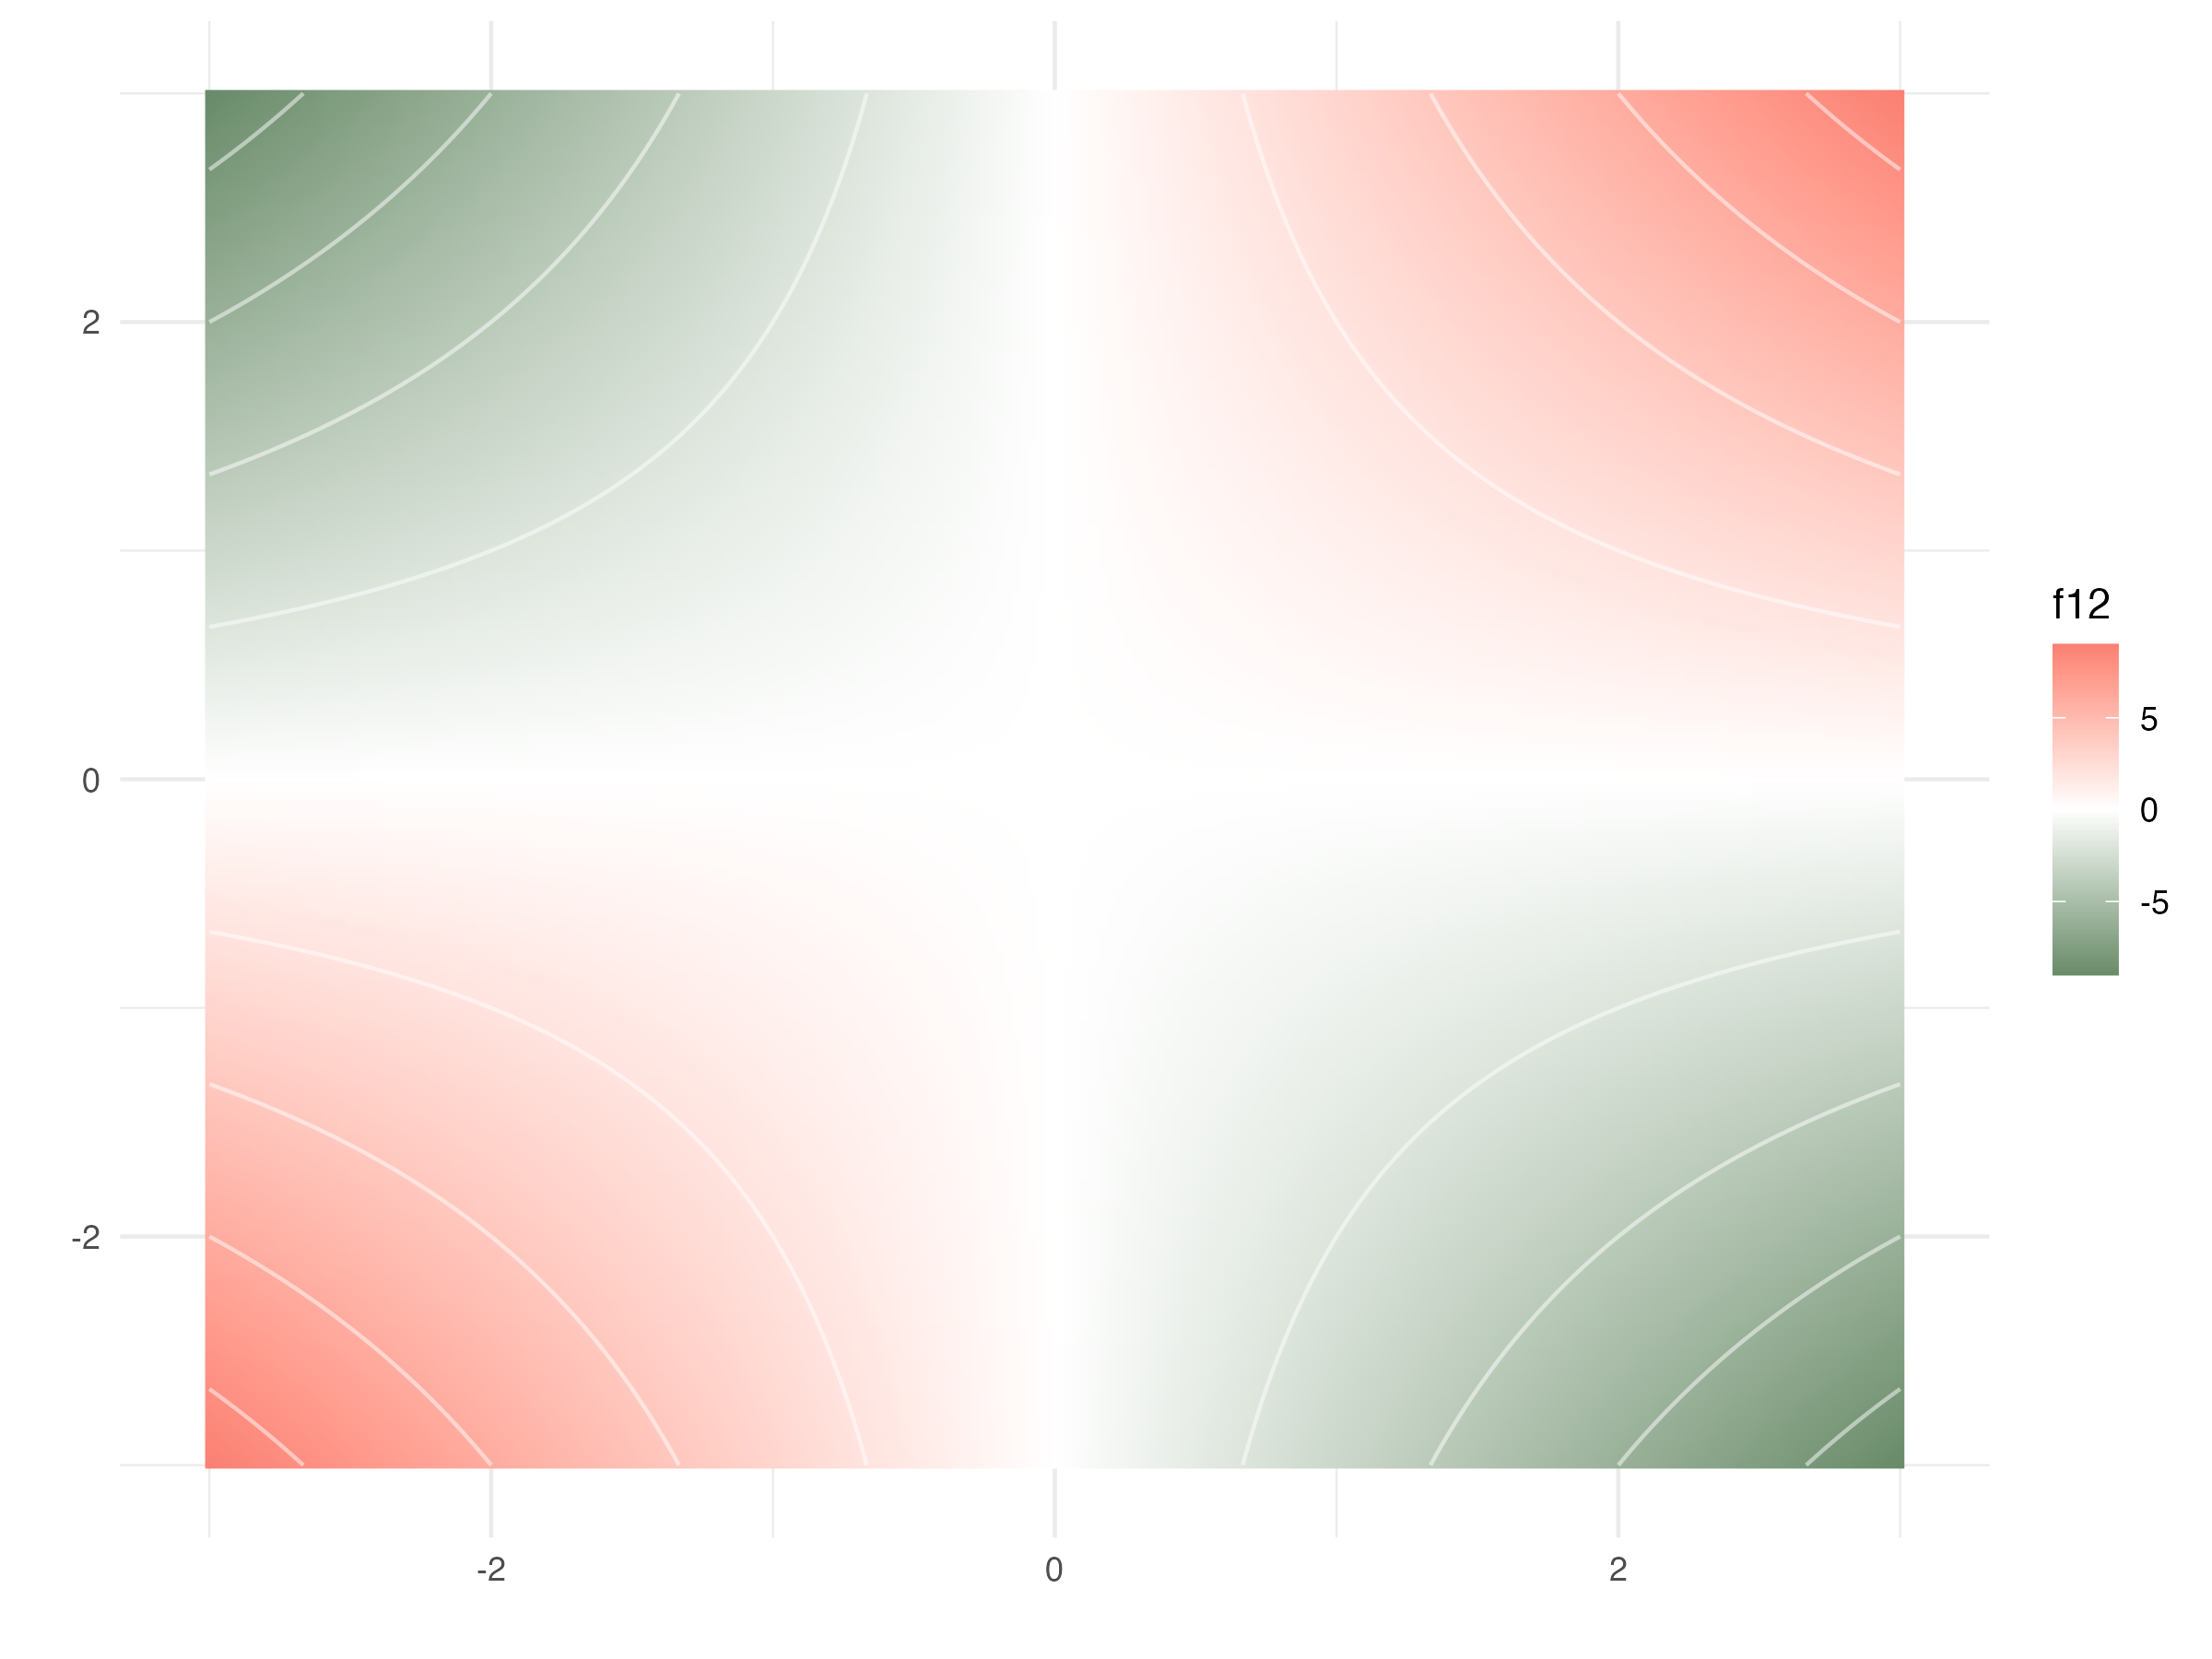
\includegraphics[width=\textwidth]{images/p_contour_ex1.png}
        \caption{Contour plot of $g(x) = x_1 + 2 x_2 + x_1 x_2$.}
        \label{fig:contour_ex1}
    \end{minipage}
\end{figure}

% Input: MVN, not centred, independent
Next, instead of a standard MVN distribution assumption for the inputs, we allow for non-centred inputs. This is to confirm that the fANOVA decomposition manages to yield zero mean components, even when inputs are not centred.
\(g = a + X_1 + 2X_2 + X_1 X_2\)
\[
\begin{pmatrix}
X_1 \\
X_2
\end{pmatrix}
\sim \mathcal{N}\left(
\begin{pmatrix} \mu_1 \\ \mu_2 \end{pmatrix},
\begin{pmatrix}
1 & 0 \\
0 & 1
\end{pmatrix}
\right).
\]
From the properties of the MVN, we know that marginal distributions are standard normal:
\[
X_i \sim \mathcal{N}(0, 1) \quad \text{for } i = 1, 2
\]

We also know that the conditional distributions are given by:
\[
X_1 \mid X_2 = x_2 \sim \mathcal{N}(\mu_1, 1), \quad
X_2 \mid X_1 = x_1 \sim \mathcal{N}(\mu_2, 1)
\]

We can now compute the classical fANOVA components as follows:
\begin{align*}
    y_{\emptyset} &= \mathbb{E}[g(X)] = a + \mu_1 + 2\mu_2 + \mu_1 \mu_2, \\
    y_1 &= \mathbb{E}[g(X) \mid X_2 = x_2] - y_{\emptyset}= a + 2\mu_2 + x_1 + x_1 \mu_2 - y_{\emptyset} \\
    &= x_1 ( 1 + \mu_2) - \mu_1 \mu_2 - \mu_1, \\
    y_2 &= \mathbb{E}[g(X) \mid X_1 = x_1] - y_{\emptyset} = a + \mu_1 + 2x_2 + x_2 \mu_1 - y_{\emptyset} \\
    &= x_2 (2 + \mu_1) - \mu_1 \mu_2 - 2 \mu_2, \\
    y_{12} &= g(x_1, x_2) - y_{\emptyset} = x_1x_2 - \mu_2 x_1 - \mu_1 x_2 + \mu_1 \mu_2.      
\end{align*}
We recognize that each fANOVA components is shifted by constants (that are formed from the conditional and unconditional expected values of the input variables). 

It is easy to verify that non-constant terms have mean zero:
\begin{align*}
    \mathbb{E}[y_1] &= \mathbb{E}[X_1 (1 + \mu_2) - \mu_1 \mu_2 - \mu_1] = (1 + \mu_2) \mathbb{E}[X_1] - \mu_1 \mu_2 - \mu_1 = 0, \\
    \mathbb{E}[y_2] &= \mathbb{E}[X_2 (2 + \mu_1) - \mu_1 \mu_2 - 2\mu_2] = (2 + \mu_1) \mathbb{E}[X_2] - \mu_1 \mu_2 - 2\mu_2 = 0, \\
    \mathbb{E}[y_{12}] &= \mathbb{E}[X_1X_2] - \mu_2 \mathbb{E}[X_1] - \mu_1 \mathbb{E}[X_2] + \mu_1 \mu_2 = 0.
\end{align*}
Varying the mean of MVN inputs will result in shifted fANOVA components. Varying the variance of intput variables will not change the fANOVA decomposition and is therefore not investigated further.
% Input: Poisson/ Exponential/ Beta/ etc. not centred, independent


\subsubsection*{Standard MVN, linear function, interaction, dependent inputs}
% Zwei Plots für rho = 0.6 nebeneinander, jeweils halbe Breite
\begin{figure}[htpb]
    \centering
    \begin{minipage}[t]{0.49\textwidth}
        \centering
        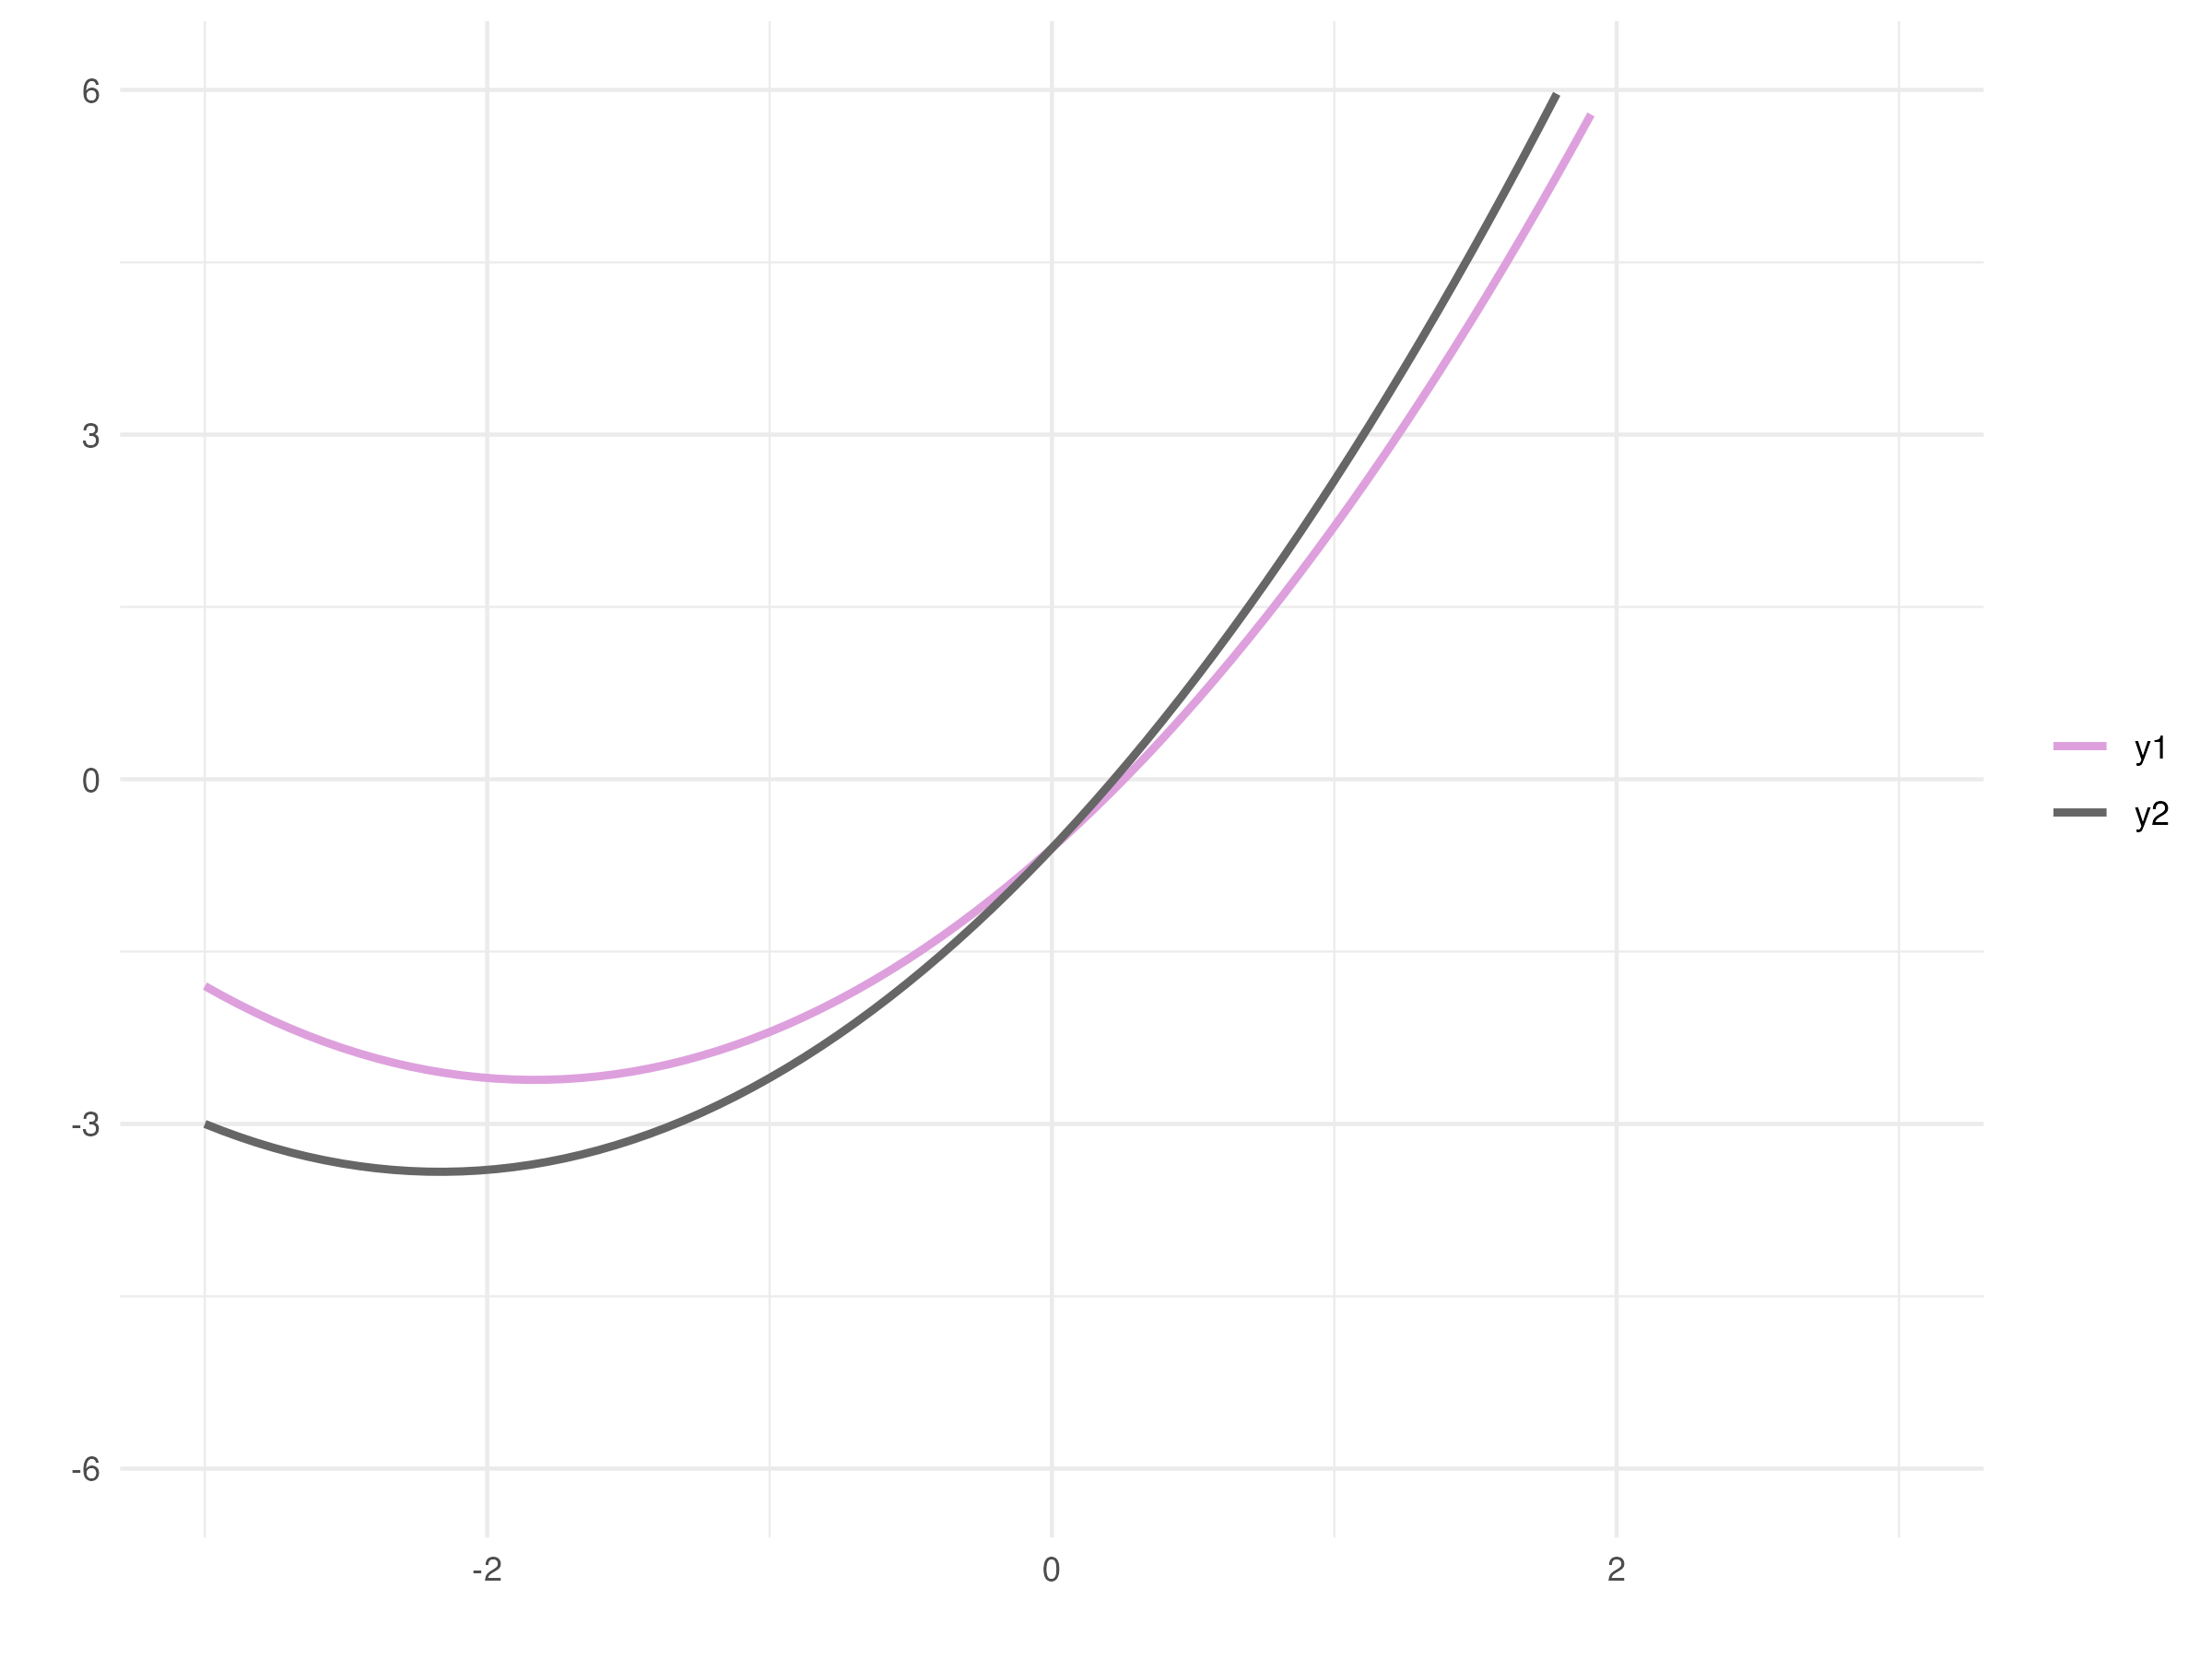
\includegraphics[width=\textwidth]{images/p_main_effect_ex1_rho06.png}
        \caption{Main terms as calculated via classical fANOVA for $g(x) = x_1 + 2 x_2 + x_1 x_2$ with $\rho = 0.6$.}
        \label{fig:main_effects_ex1_rho06}
    \end{minipage}%
    \hfill
    \begin{minipage}[t]{0.49\textwidth}
        \centering
        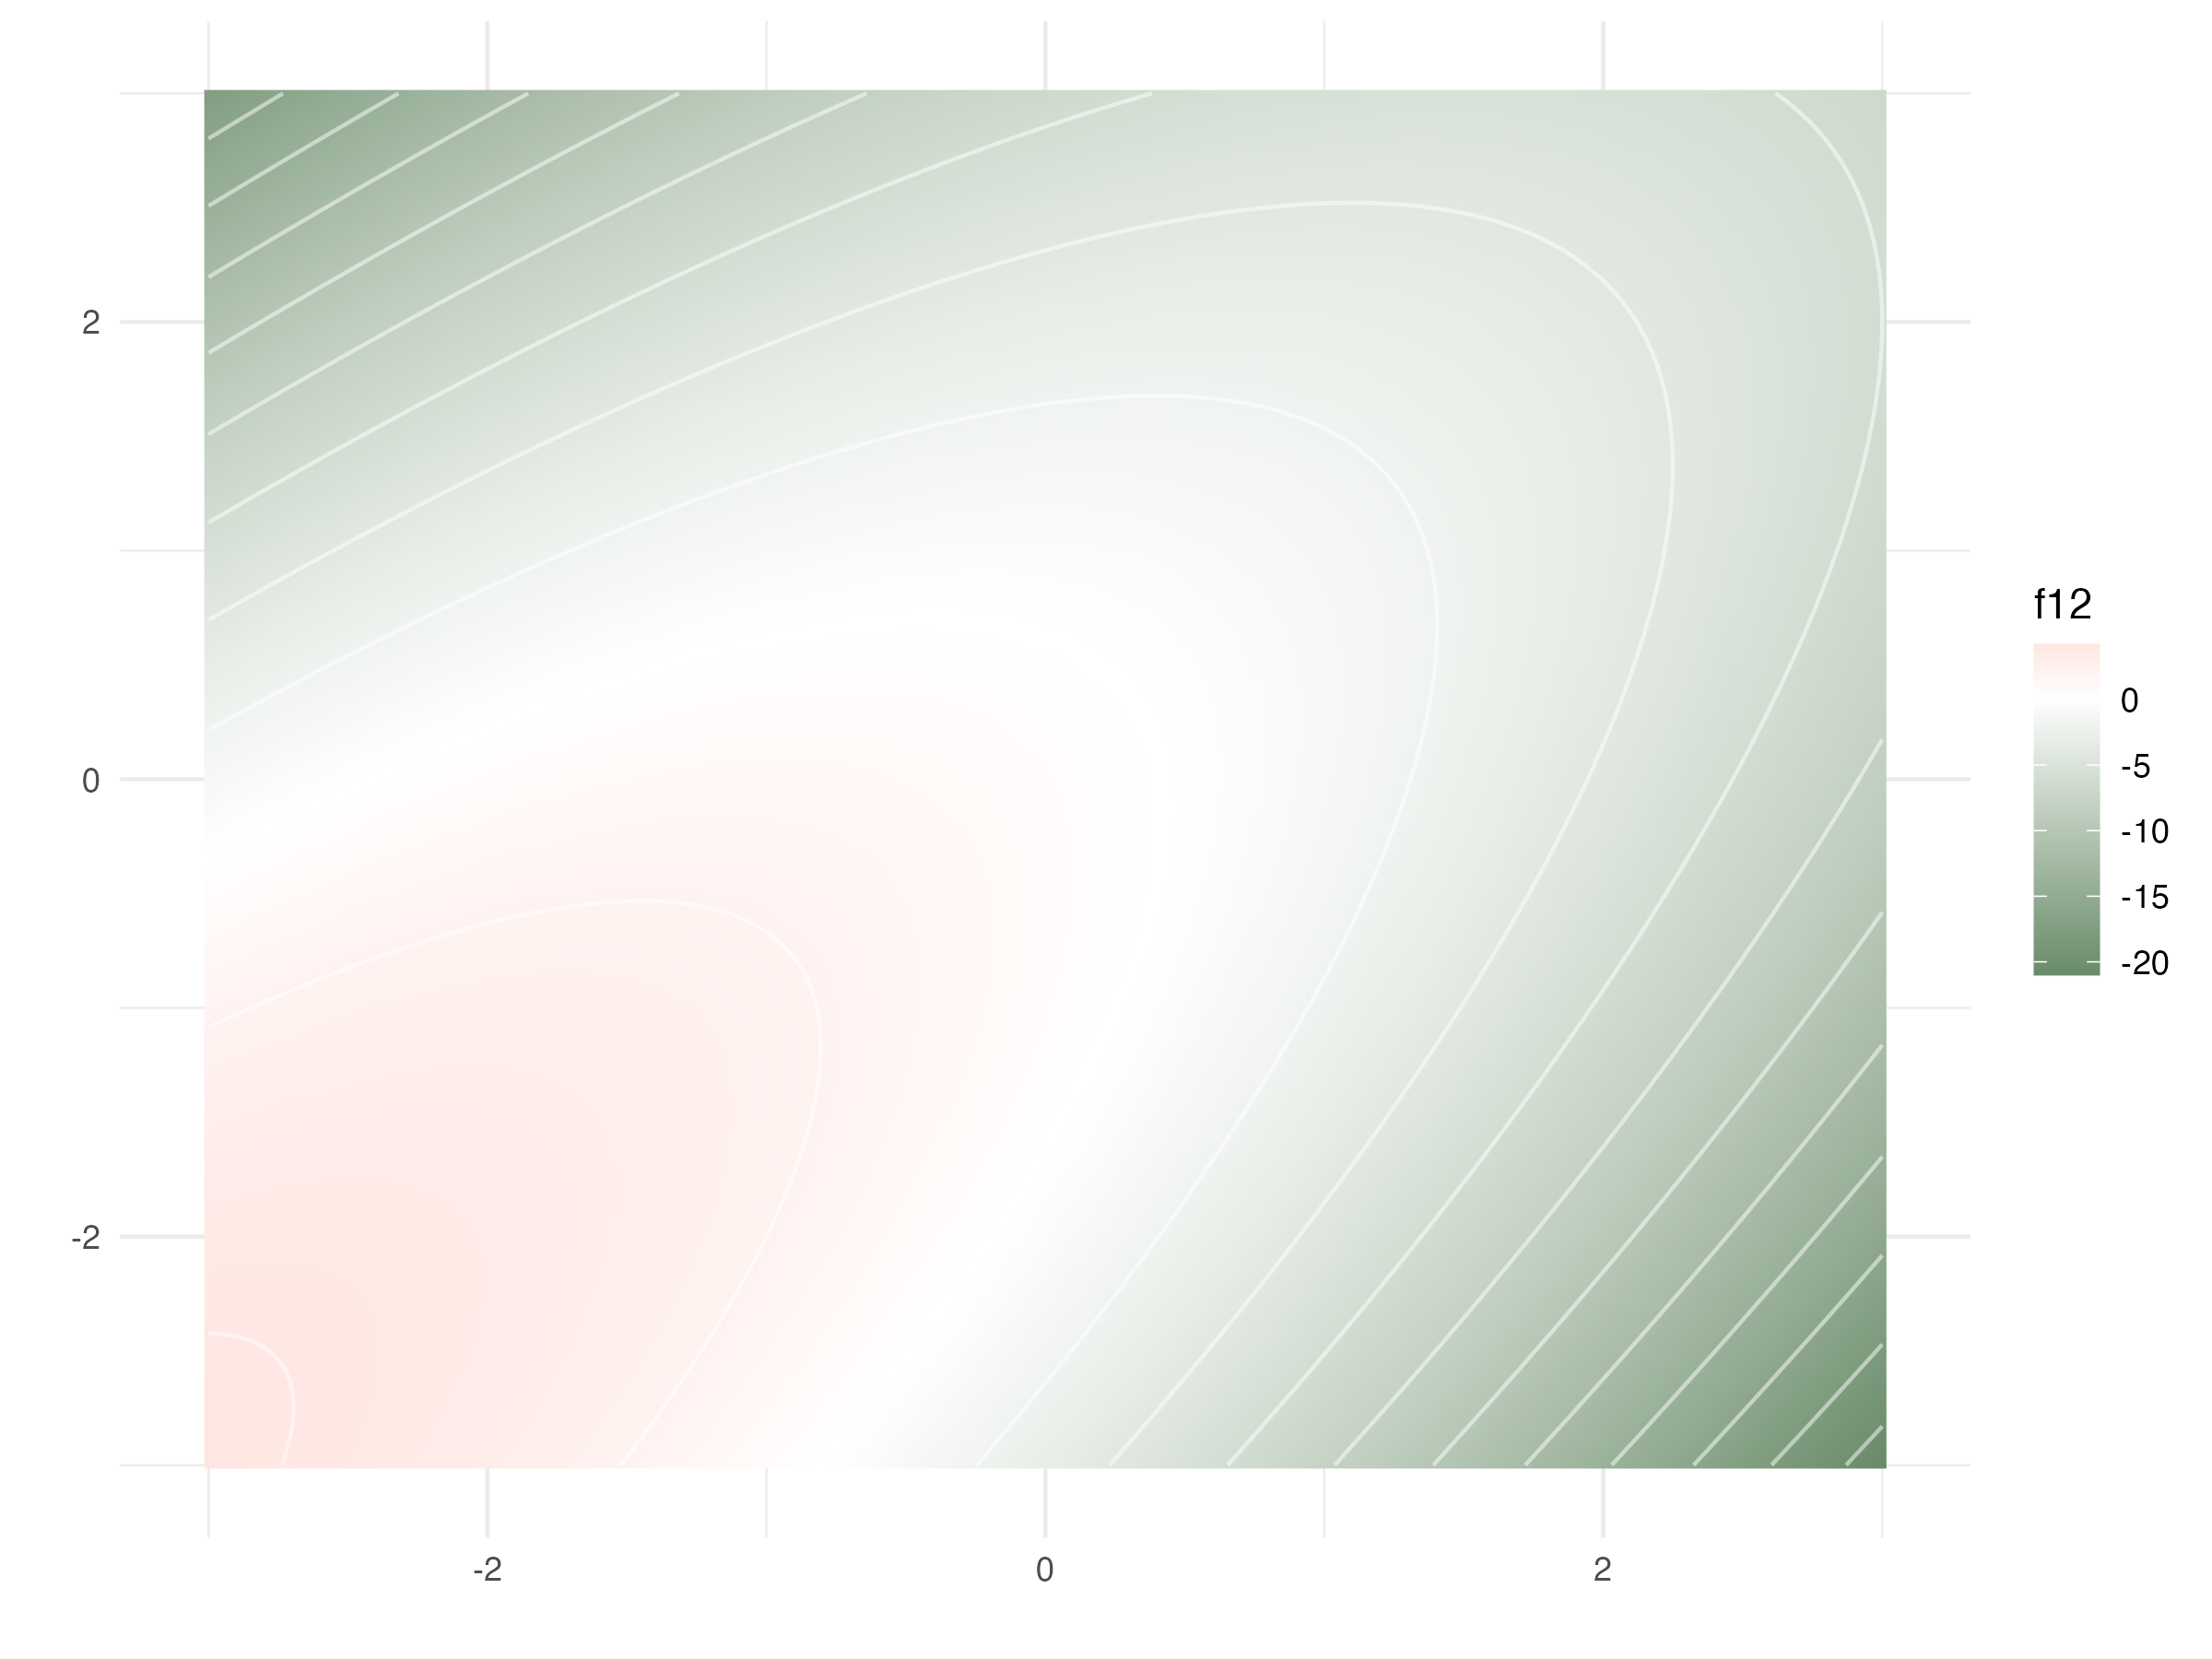
\includegraphics[width=\textwidth]{images/p_contour_ex1_rho06.png}
        \caption{Contour plot of $g(x) = x_1 + 2 x_2 + x_1 x_2$ with $\rho = 0.6$.}
        \label{fig:contour_ex1_rho06}
    \end{minipage}
\end{figure}

So \autoref{fig:main_effects_ex1_rho06} and \autoref{fig:contour_ex1_rho06} are not how we want the fANOVA components to look like under dependence - but how do we want them to look like?
Since we changed nothing about the structure of the function, should they generate identical plots as the classical components??

But on the other hand it cannot be that they give the same plots... I mean we wrote down the definition of the generalized components earlier, of course it is not the same as for the classical components. So as a function they literally look different. We couldn't compute them exactly but we could at least write out the system of equations we have to solve/ the probem that needs to be solved.

\subsubsection*{Uniform, quadratic, no interaction}
Let us also try out another function $g(x_1, x_2) = a + x_1 + x_2^2$; to see how fANOVA deals with quadratic main effects. 
We will also change the distribution of the inputs. Lets us consider two independent random variables with uniform distribution over the interval \([-1, 1]\), meaning they are already centred. We calculate:
\begin{align*}
y_\emptyset &= \mathbb{E}[g(X_1, X_2)] = a + \mathbb{E}[X_1] + \mathbb{E}[X_2^2] = a + 0 + \tfrac{1}{3} = a + \tfrac{1}{3} \\
y_1(x_1) &= \mathbb{E}[g(x_1, X_2)] - y_\emptyset = a + x_1 + \tfrac{1}{3} - \left(a + \tfrac{1}{3}\right) = x_1 \\
y_2(x_2) &= \mathbb{E}[g(X_1, x_2)] - y_\emptyset = a + 0 + x_2^2 - \left(a + \tfrac{1}{3}\right) = x_2^2 - \tfrac{1}{3} \\
y_{1,2}(x_1, x_2) &= g(x_1, x_2) - y_\emptyset - y_1(x_1) - y_2(x_2) = a + x_1 + x_2^2 - \left(a + \tfrac{1}{3} + x_1 + x_2^2 - \tfrac{1}{3}\right) = 0
\end{align*}
